\documentclass[en]{../../../eplexercises}

\usetikzlibrary{shapes}

\newcommand{\cloud}[4]{\node [cloud, draw,cloud puffs=10,cloud puff arc=120, aspect=2, minimum width=#3cm, minimum height=#4cm] at (#1,#2) {};}
% \node{Xcenter}{Ycenter}{width}{height} make a cloud

\newcommand{\router}[3]{\node[draw,rectangle,rounded corners=5pt] (#1) at (#2,#3) {#1};}
% \router{name}{Xcenter}{Ycenter} make a router
\newcommand{\routerRR}[4]{\node[draw,rectangle,rounded corners=5pt] (#1) at (#2,#3) {#1};\node[draw,circle,minimum height=#4cm,blue, very thick] at (#2,#3) {};}
% \routerRR{name}{Xcenter}{Ycenter}{height} height is the size of the circle that round that router

\newcommand{\link}[2]{\draw[thick] (#1) -- (#2);}
% \link{name1}{name2} create a link between the routers name1 and name2

\newcommand{\linkIGP}[3]{\draw[thick] (#1) -- node[sloped,midway,above] {IGP=#3} (#2);}
% \linkIGP{name1}{name2}{weight} create a IGP link between the routers name1 and name 2 with a IGP weigth of weight (display the IGP weith above the link)
\newcommand{\linkIGPdown}[3]{\draw[thick] (#1) -- node[sloped,midway,below] {IGP=#3} (#2);}
% \linkIGPdown{name1}{name2}{weight} create a IGP link between the routers name1 and name 2 with a IGP weigth of weight (!!display the IGP weith under the link)

\newcommand{\linkeBGP}[2]{\draw[thick,red,<->,>=latex] (#1) -- (#2);}
% \linkeBGP{name1}{name2} create an eBGP link between the routers name1 and name2
\newcommand{\linkeBGPMED}[3]{\draw[thick,red,<->,>=latex] (#1) -- node[midway,above,sloped] {\color{red}{MED=#3}} (#2);}
% \linkeBGPMED{name1}{name2}{weight} create an eBGP link between the routers name1 and name 2 with a MED weigth of weight (display the MED weith above the link)
\newcommand{\linkeBGPMEDdown}[3]{\draw[thick,red,<->,>=latex] (#1) -- node[midway,below,sloped] {\color{red}{MED=#3}} (#2);}
% \linkeBGPMEDdown{name1}{name2}{weight} create an eBGP link between the routers name1 and name 2 with a MED weigth of weight (!!display the MED weith under the link)

\hypertitle{Computer networks: configuration and management}{7}{INGI}{2142}
{Luis Tascon Gutierrez}
{Olivier Bonaventure}

\newpage
\section{iBGP}
\subsection{Slide 22}
Write the BGP routes towards prefix p on all routers inside AS1.
\begin{center}
    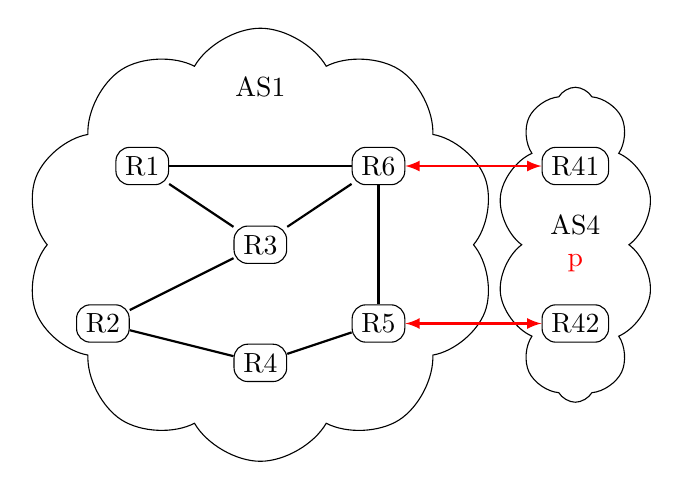
\begin{tikzpicture}
    \node at (0,2) {AS1}; \node[above] at (4,0) {AS4}; \node[below] at (4,0) {\color{red}{p}};
    \cloud{0}{0}{6}{5.5}    \router{R1}{-1.5}{1}
    \router{R6}{1.5}{1}    \router{R3}{0}{0}
    \router{R2}{-2}{-1}    \router{R4}{0}{-1.5}
    \router{R5}{1.5}{-1}
    \link{R1}{R6}\link{R1}{R3}\link{R3}{R6}\link{R3}{R2}
    \link{R2}{R4}\link{R4}{R5}\link{R5}{R6}
    \cloud{4}{0}{2}{4}    \router{R41}{4}{1}
    \router{R42}{4}{-1}
    \linkeBGP{R6}{R41}\linkeBGP{R5}{R42}
    \end{tikzpicture}
\end{center}
\begin{solution}
\begin{tabular}{rl|rl|rl}
    \multirow{2}{*}{R1} & *p,AS4,R6,1 & \multirow{2}{*}{R2} & *p,AS4,R5,2 & \multirow{2}{*}{R3} & *p,AS4,R6,1\\
    & p,AS4,R5,2 & & p,AS4,R6,2 & & p,AS4,R5,2\\
    \hline
     \multirow{2}{*}{R4} & *p,AS4,R5,1 & \multirow{2}{*}{R5} & *p,AS4,R5,0 & \multirow{2}{*}{R6} & *p,AS4,R6,0\\
      & p,AS4,R6,2 & & p,AS4,R6,1 & & p,AS4,R5,1\\
\end{tabular}
\end{solution}

\subsection{Slide 23}
Write the BGP routes towards prefix p on all routers inside AS1.
\begin{center}
    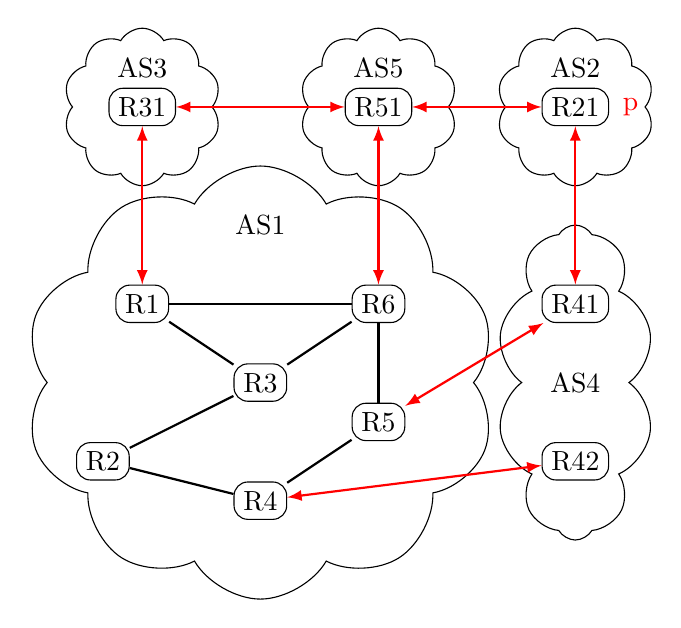
\begin{tikzpicture}
    \node at (0,2) {AS1}; \node at (4,0) {AS4}; 
    \cloud{0}{0}{6}{5.5}    \router{R1}{-1.5}{1}
    \router{R6}{1.5}{1}    \router{R3}{0}{0}
    \router{R2}{-2}{-1}    \router{R4}{0}{-1.5}
    \router{R5}{1.5}{-0.5}
    \link{R1}{R6}\link{R1}{R3}\link{R3}{R6}\link{R3}{R2}
    \link{R2}{R4}\link{R4}{R5}\link{R5}{R6}
    \cloud{4}{0}{2}{4}    \router{R41}{4}{1}
    \router{R42}{4}{-1}
    \linkeBGP{R5}{R41}\linkeBGP{R4}{R42}
    
    \cloud{-1.5}{3.5}{2}{2} \router{R31}{-1.5}{3.5} \node at (-1.5,4) {AS3};
    \cloud{1.5}{3.5}{2}{2} \router{R51}{1.5}{3.5} \node at (1.5,4) {AS5};
    \cloud{4}{3.5}{2}{2} \router{R21}{4}{3.5} \node at (4,4) {AS2}; \node at (4.7,3.5) {\color{red}{p}};
    \linkeBGP{R1}{R31} \linkeBGP{R6}{R51} \linkeBGP{R31}{R51} \linkeBGP{R51}{R21} \linkeBGP{R21}{R41}
    \end{tikzpicture}
\end{center}
\nosolution

\subsection{Slide 25}
Write the BGP routes towards prefix p on all routers inside AS1.
\begin{center}
    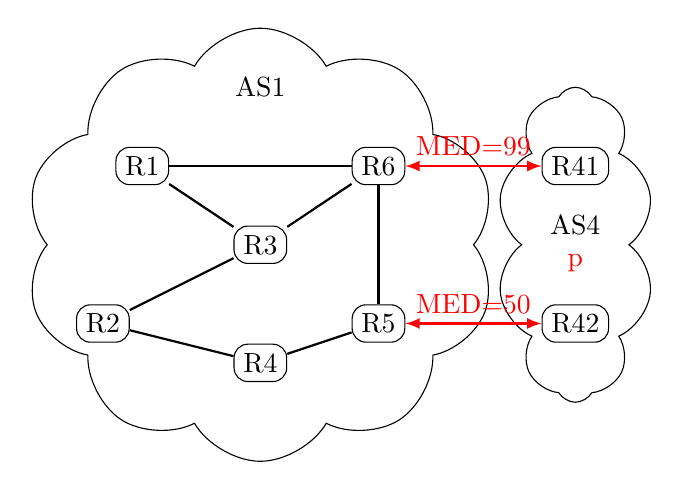
\begin{tikzpicture}
    \node at (0,2) {AS1}; \node[above] at (4,0) {AS4}; \node[below] at (4,0) {\color{red}{p}};
    \cloud{0}{0}{6}{5.5}    \router{R1}{-1.5}{1}
    \router{R6}{1.5}{1}    \router{R3}{0}{0}
    \router{R2}{-2}{-1}    \router{R4}{0}{-1.5}
    \router{R5}{1.5}{-1}
    \link{R1}{R6}\link{R1}{R3}\link{R3}{R6}\link{R3}{R2}
    \link{R2}{R4}\link{R4}{R5}\link{R5}{R6}
    \cloud{4}{0}{2}{4}    \router{R41}{4}{1}
    \router{R42}{4}{-1}
    \linkeBGPMED{R6}{R41}{99}\linkeBGPMED{R5}{R42}{50}
    \end{tikzpicture}
\end{center}
\nosolution

\subsection{Slide 26}
Write the BGP routes towards prefix p on all routers inside AS1.
\begin{center}
    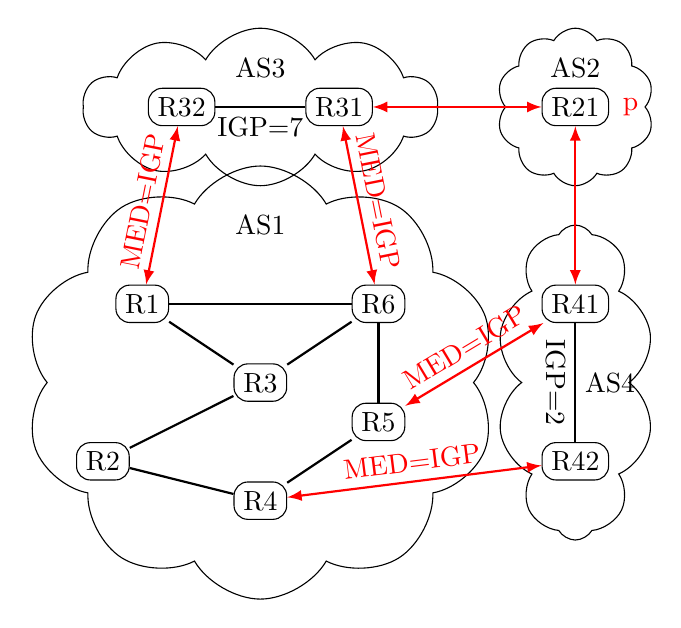
\begin{tikzpicture}
    \node at (0,2) {AS1}; \node[right] at (4,0) {AS4}; 
    \cloud{0}{0}{6}{5.5}    \router{R1}{-1.5}{1}
    \router{R6}{1.5}{1}    \router{R3}{0}{0}
    \router{R2}{-2}{-1}    \router{R4}{0}{-1.5}
    \router{R5}{1.5}{-0.5}
    \link{R1}{R6}\link{R1}{R3}\link{R3}{R6}\link{R3}{R2}
    \link{R2}{R4}\link{R4}{R5}\link{R5}{R6}
    \cloud{4}{0}{2}{4}    \router{R41}{4}{1}
    \router{R42}{4}{-1} \linkIGPdown{R41}{R42}{2}
    \linkeBGPMED{R5}{R41}{IGP}\linkeBGPMED{R4}{R42}{IGP}
    
    \cloud{0}{3.5}{4.5}{2} \router{R32}{-1}{3.5} \node at (0,4) {AS3};\router{R31}{1}{3.5}
    \cloud{4}{3.5}{2}{2} \router{R21}{4}{3.5} \node at (4,4) {AS2}; \node at (4.7,3.5) {\color{red}{p}};
    \linkeBGPMED{R1}{R32}{IGP} \linkeBGPMED{R6}{R31}{IGP} 
    \linkeBGP{R21}{R41} \linkeBGP{R31}{R21}
    \linkIGPdown{R32}{R31}{7}
    \end{tikzpicture}
\end{center}
\nosolution

\subsection{Slide 32}
What happens if iBGP session are missing? Write the BGP routes towards prefix p on all routers inside AS1.
\begin{center}
    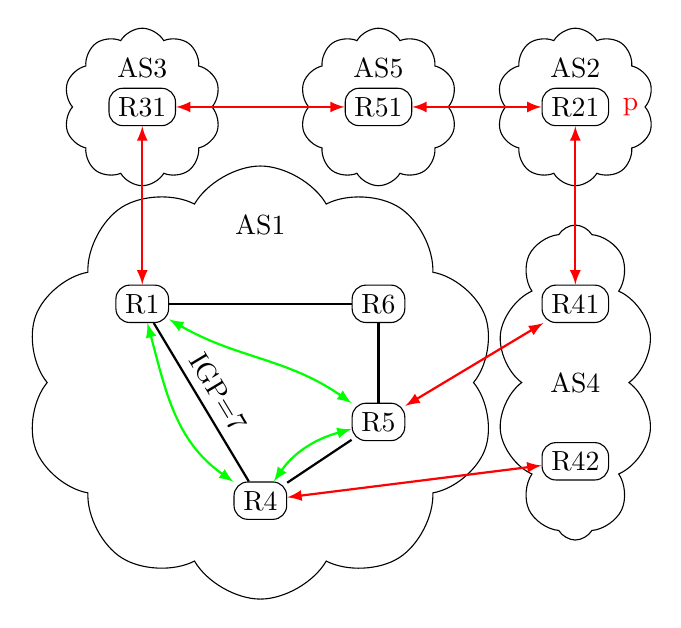
\begin{tikzpicture}
    \node at (0,2) {AS1}; \node at (4,0) {AS4}; 
    \cloud{0}{0}{6}{5.5}    \router{R1}{-1.5}{1}
    \router{R6}{1.5}{1}   
    \router{R4}{0}{-1.5}    \router{R5}{1.5}{-0.5}
    \link{R1}{R6}\linkIGP{R1}{R4}{7}
    \link{R4}{R5}\link{R5}{R6}
    \cloud{4}{0}{2}{4}    \router{R41}{4}{1}
    \router{R42}{4}{-1}
    \linkeBGP{R5}{R41}\linkeBGP{R4}{R42}
    
    \cloud{-1.5}{3.5}{2}{2} \router{R31}{-1.5}{3.5} \node at (-1.5,4) {AS3};
    \cloud{1.5}{3.5}{2}{2} \router{R51}{1.5}{3.5} \node at (1.5,4) {AS5};
    \cloud{4}{3.5}{2}{2} \router{R21}{4}{3.5} \node at (4,4) {AS2}; \node at (4.7,3.5) {\color{red}{p}};
    \linkeBGP{R1}{R31}  \linkeBGP{R31}{R51} \linkeBGP{R51}{R21} \linkeBGP{R21}{R41}
    \draw[green,<->,>=latex,thick] (R1) to[out=-75,in=145] (R4);
    \draw[green,<->,>=latex,thick] (R1) to[out=-30,in=145] (R5);
    \draw[green,<->,>=latex,thick] (R4) to[out=55,in=-165] (R5);
    \end{tikzpicture}
\end{center}
\nosolution

\subsection{Slide 33}
What happens if iBGP session are missing? Write the BGP routes towards prefix p on all routers inside AS1.
\begin{center}
    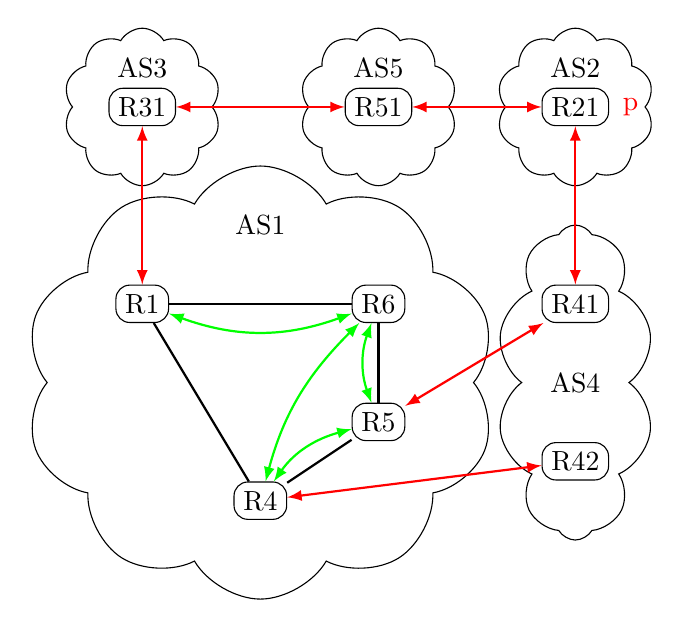
\begin{tikzpicture}
    \node at (0,2) {AS1}; \node at (4,0) {AS4}; 
    \cloud{0}{0}{6}{5.5}    \router{R1}{-1.5}{1}
    \router{R6}{1.5}{1}   
    \router{R4}{0}{-1.5}    \router{R5}{1.5}{-0.5}
    \link{R1}{R6}\link{R1}{R4}
    \link{R4}{R5}\link{R5}{R6}
    \cloud{4}{0}{2}{4}    \router{R41}{4}{1}
    \router{R42}{4}{-1}
    \linkeBGP{R5}{R41}\linkeBGP{R4}{R42}
    
    \cloud{-1.5}{3.5}{2}{2} \router{R31}{-1.5}{3.5} \node at (-1.5,4) {AS3};
    \cloud{1.5}{3.5}{2}{2} \router{R51}{1.5}{3.5} \node at (1.5,4) {AS5};
    \cloud{4}{3.5}{2}{2} \router{R21}{4}{3.5} \node at (4,4) {AS2}; \node at (4.7,3.5) {\color{red}{p}};
    \linkeBGP{R1}{R31}  \linkeBGP{R31}{R51} \linkeBGP{R51}{R21} \linkeBGP{R21}{R41}
    \draw[green,thick,<->,>=latex] (R1) to[out=-20,in=-160] (R6);
    \draw[green,thick,<->,>=latex] (R4) to[out=75,in=-135] (R6);
    \draw[green,thick,<->,>=latex] (R5) to[out=110,in=-110] (R6);
    \draw[green,thick,<->,>=latex] (R4) to[out=55,in=-165] (R5);
    \end{tikzpicture}
\end{center}
\nosolution

\subsection{Slide 34}
What happens if iBGP session are missing? Write the BGP routes towards prefix p on all routers inside AS1.
\begin{center}
    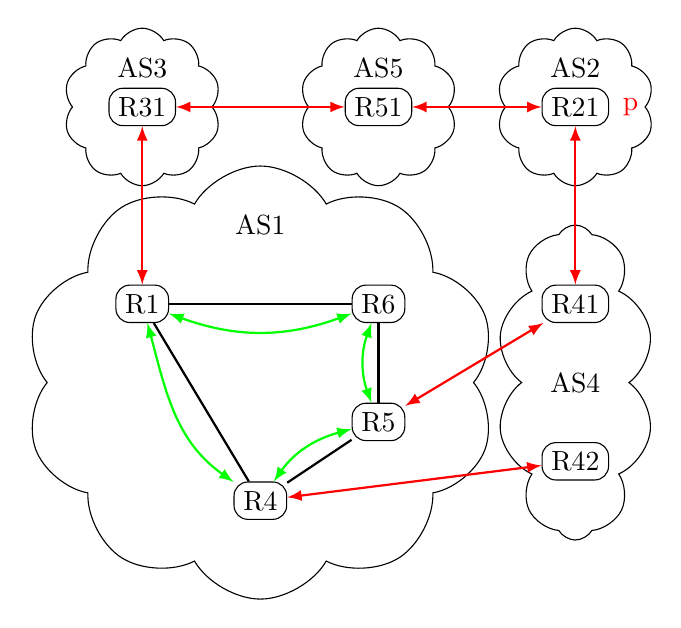
\begin{tikzpicture}
    \node at (0,2) {AS1}; \node at (4,0) {AS4}; 
    \cloud{0}{0}{6}{5.5}    \router{R1}{-1.5}{1}
    \router{R6}{1.5}{1}   
    \router{R4}{0}{-1.5}    \router{R5}{1.5}{-0.5}
    \link{R1}{R6}\link{R1}{R4}
    \link{R4}{R5}\link{R5}{R6}
    \cloud{4}{0}{2}{4}    \router{R41}{4}{1}
    \router{R42}{4}{-1}
    \linkeBGP{R5}{R41}\linkeBGP{R4}{R42}
    
    \cloud{-1.5}{3.5}{2}{2} \router{R31}{-1.5}{3.5} \node at (-1.5,4) {AS3};
    \cloud{1.5}{3.5}{2}{2} \router{R51}{1.5}{3.5} \node at (1.5,4) {AS5};
    \cloud{4}{3.5}{2}{2} \router{R21}{4}{3.5} \node at (4,4) {AS2}; \node at (4.7,3.5) {\color{red}{p}};
    \linkeBGP{R1}{R31}  \linkeBGP{R31}{R51} \linkeBGP{R51}{R21} \linkeBGP{R21}{R41}
    \draw[green,<->,>=latex,thick] (R1) to[out=-75,in=145] (R4);
    \draw[green,thick,<->,>=latex] (R1) to[out=-20,in=-160] (R6);
    \draw[green,thick,<->,>=latex] (R5) to[out=110,in=-110] (R6);
    \draw[green,thick,<->,>=latex] (R4) to[out=55,in=-165] (R5);
    \end{tikzpicture}
\end{center}
\nosolution

\subsection{Slide 38}
With Route Reflector: Write the BGP routes towards prefix p on all routers inside AS1.
\begin{center}
    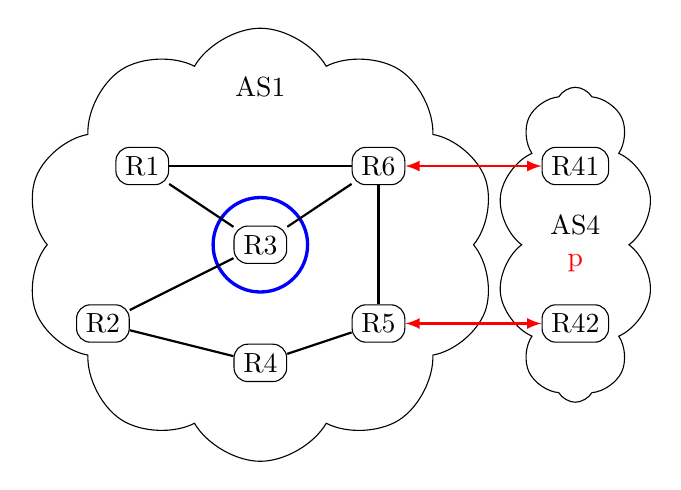
\begin{tikzpicture}
    \node at (0,2) {AS1}; \node[above] at (4,0) {AS4}; \node[below] at (4,0) {\color{red}{p}};
    \cloud{0}{0}{6}{5.5}    \router{R1}{-1.5}{1}
    \router{R6}{1.5}{1}    \routerRR{R3}{0}{0}{1.2}
    \router{R2}{-2}{-1}    \router{R4}{0}{-1.5}
    \router{R5}{1.5}{-1}
    \link{R1}{R6}\link{R1}{R3}\link{R3}{R6}\link{R3}{R2}
    \link{R2}{R4}\link{R4}{R5}\link{R5}{R6}
    \cloud{4}{0}{2}{4}    \router{R41}{4}{1}
    \router{R42}{4}{-1}
    \linkeBGP{R6}{R41}\linkeBGP{R5}{R42}
    \end{tikzpicture}
\end{center}
\nosolution

\subsection{Slide 39}
With Route Reflector: Write the BGP routes towards prefix p on all routers inside AS1.
\begin{center}
    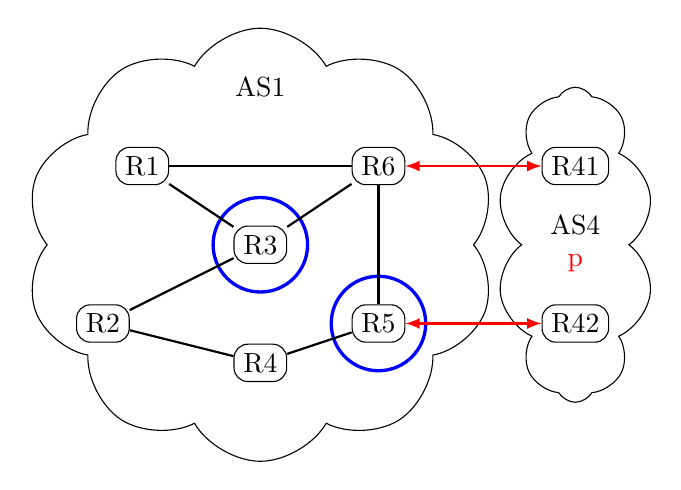
\begin{tikzpicture}
    \node at (0,2) {AS1}; \node[above] at (4,0) {AS4}; \node[below] at (4,0) {\color{red}{p}};
    \cloud{0}{0}{6}{5.5}    \router{R1}{-1.5}{1}
    \router{R6}{1.5}{1}    \routerRR{R3}{0}{0}{1.2}
    \router{R2}{-2}{-1}    \router{R4}{0}{-1.5}
    \routerRR{R5}{1.5}{-1}{1.2}
    \link{R1}{R6}\link{R1}{R3}\link{R3}{R6}\link{R3}{R2}
    \link{R2}{R4}\link{R4}{R5}\link{R5}{R6}
    \cloud{4}{0}{2}{4}    \router{R41}{4}{1}
    \router{R42}{4}{-1}
    \linkeBGP{R6}{R41}\linkeBGP{R5}{R42}
    \end{tikzpicture}
\end{center}
\nosolution

\subsection{Slide 40}
With Route Reflector: Write the BGP routes towards prefix p on all routers inside AS1.
\begin{center}
    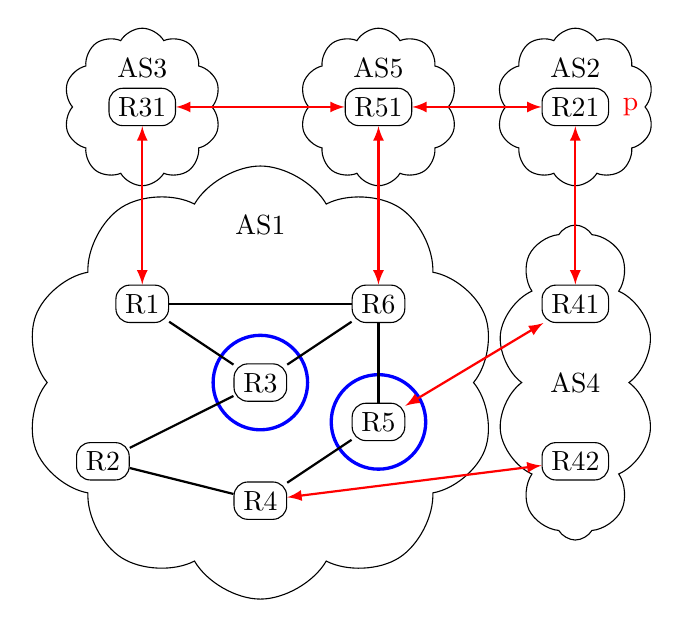
\begin{tikzpicture}
    \node at (0,2) {AS1}; \node at (4,0) {AS4}; 
    \cloud{0}{0}{6}{5.5}    \router{R1}{-1.5}{1}
    \router{R6}{1.5}{1}    \routerRR{R3}{0}{0}{1.2}
    \router{R2}{-2}{-1}    \router{R4}{0}{-1.5}
    \routerRR{R5}{1.5}{-0.5}{1.2}
    \link{R1}{R6}\link{R1}{R3}\link{R3}{R6}\link{R3}{R2}
    \link{R2}{R4}\link{R4}{R5}\link{R5}{R6}
    \cloud{4}{0}{2}{4}    \router{R41}{4}{1}
    \router{R42}{4}{-1}
    \linkeBGP{R5}{R41}\linkeBGP{R4}{R42}
    
    \cloud{-1.5}{3.5}{2}{2} \router{R31}{-1.5}{3.5} \node at (-1.5,4) {AS3};
    \cloud{1.5}{3.5}{2}{2} \router{R51}{1.5}{3.5} \node at (1.5,4) {AS5};
    \cloud{4}{3.5}{2}{2} \router{R21}{4}{3.5} \node at (4,4) {AS2}; \node at (4.7,3.5) {\color{red}{p}};
    \linkeBGP{R1}{R31} \linkeBGP{R6}{R51} \linkeBGP{R31}{R51} \linkeBGP{R51}{R21} \linkeBGP{R21}{R41}
    \end{tikzpicture}
\end{center}
\nosolution

\subsection{Slide 41}
With Route Reflector: What is the best place for a single route reflector?
\begin{center}
    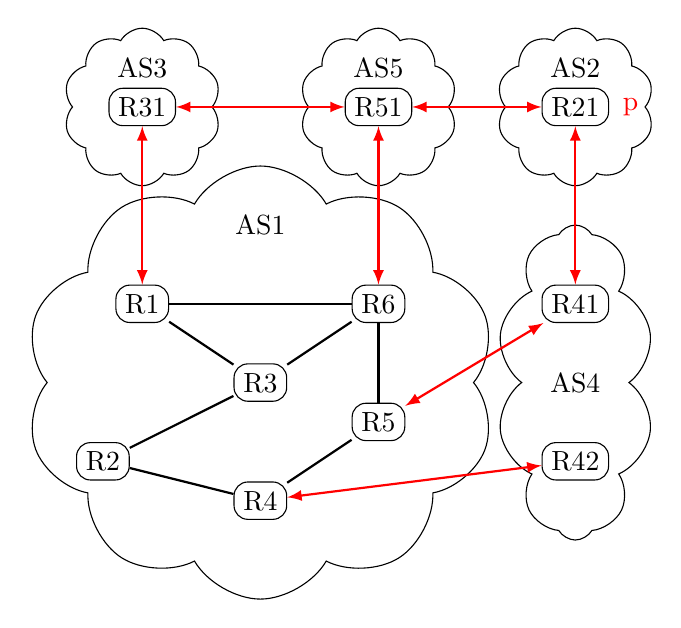
\begin{tikzpicture}
    \node at (0,2) {AS1}; \node at (4,0) {AS4}; 
    \cloud{0}{0}{6}{5.5}    \router{R1}{-1.5}{1}
    \router{R6}{1.5}{1}    \router{R3}{0}{0}
    \router{R2}{-2}{-1}    \router{R4}{0}{-1.5}
    \router{R5}{1.5}{-0.5}
    \link{R1}{R6}\link{R1}{R3}\link{R3}{R6}\link{R3}{R2}
    \link{R2}{R4}\link{R4}{R5}\link{R5}{R6}
    \cloud{4}{0}{2}{4}    \router{R41}{4}{1}
    \router{R42}{4}{-1}
    \linkeBGP{R5}{R41}\linkeBGP{R4}{R42}
    
    \cloud{-1.5}{3.5}{2}{2} \router{R31}{-1.5}{3.5} \node at (-1.5,4) {AS3};
    \cloud{1.5}{3.5}{2}{2} \router{R51}{1.5}{3.5} \node at (1.5,4) {AS5};
    \cloud{4}{3.5}{2}{2} \router{R21}{4}{3.5} \node at (4,4) {AS2}; \node at (4.7,3.5) {\color{red}{p}};
    \linkeBGP{R1}{R31} \linkeBGP{R6}{R51} \linkeBGP{R31}{R51} \linkeBGP{R51}{R21} \linkeBGP{R21}{R41}
    \end{tikzpicture}
\end{center}
\nosolution

\subsection{Slide 42}
With Route Reflector: What is the best place for rwo route reflectors?
\begin{center}
    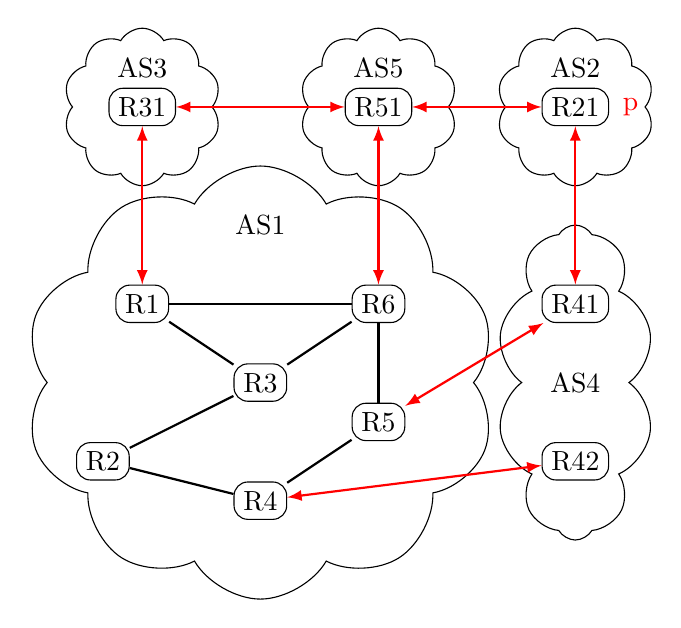
\begin{tikzpicture}
    \node at (0,2) {AS1}; \node at (4,0) {AS4}; 
    \cloud{0}{0}{6}{5.5}    \router{R1}{-1.5}{1}
    \router{R6}{1.5}{1}    \router{R3}{0}{0}
    \router{R2}{-2}{-1}    \router{R4}{0}{-1.5}
    \router{R5}{1.5}{-0.5}
    \link{R1}{R6}\link{R1}{R3}\link{R3}{R6}\link{R3}{R2}
    \link{R2}{R4}\link{R4}{R5}\link{R5}{R6}
    \cloud{4}{0}{2}{4}    \router{R41}{4}{1}
    \router{R42}{4}{-1}
    \linkeBGP{R5}{R41}\linkeBGP{R4}{R42}
    
    \cloud{-1.5}{3.5}{2}{2} \router{R31}{-1.5}{3.5} \node at (-1.5,4) {AS3};
    \cloud{1.5}{3.5}{2}{2} \router{R51}{1.5}{3.5} \node at (1.5,4) {AS5};
    \cloud{4}{3.5}{2}{2} \router{R21}{4}{3.5} \node at (4,4) {AS2}; \node at (4.7,3.5) {\color{red}{p}};
    \linkeBGP{R1}{R31} \linkeBGP{R6}{R51} \linkeBGP{R31}{R51} \linkeBGP{R51}{R21} \linkeBGP{R21}{R41}
    \end{tikzpicture}
\end{center}
\nosolution

\subsection{Slide 43}
With Route Reflector: Write the BGP routes towards prefix p on all routers inside AS1.
\begin{center}
    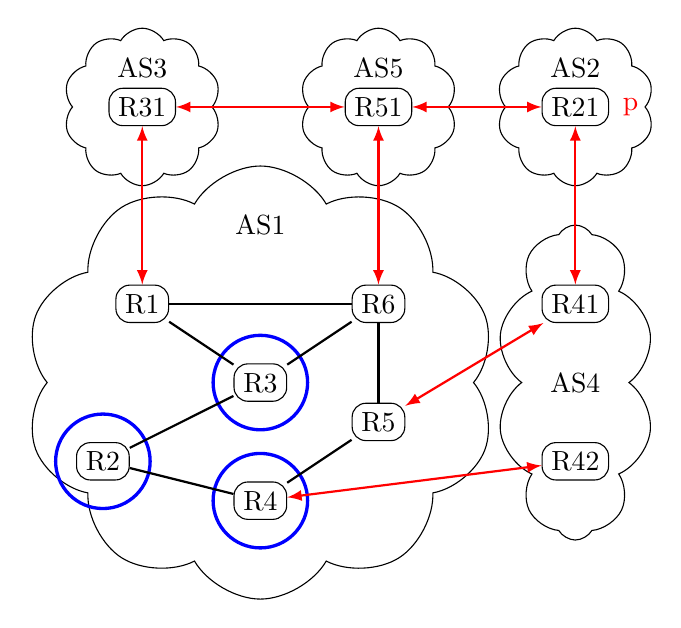
\begin{tikzpicture}
    \node at (0,2) {AS1}; \node at (4,0) {AS4}; 
    \cloud{0}{0}{6}{5.5}    \router{R1}{-1.5}{1}
    \router{R6}{1.5}{1}    \routerRR{R3}{0}{0}{1.2}
    \routerRR{R2}{-2}{-1}{1.2}    \routerRR{R4}{0}{-1.5}{1.2}
    \router{R5}{1.5}{-0.5}
    \link{R1}{R6}\link{R1}{R3}\link{R3}{R6}\link{R3}{R2}
    \link{R2}{R4}\link{R4}{R5}\link{R5}{R6}
    \cloud{4}{0}{2}{4}    \router{R41}{4}{1}
    \router{R42}{4}{-1}
    \linkeBGP{R5}{R41}\linkeBGP{R4}{R42}
    
    \cloud{-1.5}{3.5}{2}{2} \router{R31}{-1.5}{3.5} \node at (-1.5,4) {AS3};
    \cloud{1.5}{3.5}{2}{2} \router{R51}{1.5}{3.5} \node at (1.5,4) {AS5};
    \cloud{4}{3.5}{2}{2} \router{R21}{4}{3.5} \node at (4,4) {AS2}; \node at (4.7,3.5) {\color{red}{p}};
    \linkeBGP{R1}{R31} \linkeBGP{R6}{R51} \linkeBGP{R31}{R51} \linkeBGP{R51}{R21} \linkeBGP{R21}{R41}
    \end{tikzpicture}
\end{center}
\nosolution

\end{document}
